
  % Ohm's Law
  \newsavebox{\ohmbox}
  \begin{lrbox}{\ohmbox}
    \begin{tikzpicture}
      
\draw (0,0) node[anchor=south] (a) {A}
to[R=$R$,v=$v_{AB}$,f=$i$] ++(0,-2) node[anchor=north] (b)
{B};

\node[anchor=west] at ($(a)!0.5!(b)+(1,0)$) {%
$\begin{aligned}%
    v_{AB} &= iR\\
    v_A &= v_B + iR\\%
    i &= \frac{v_{AB}}{R}\\
    i &= \frac{v_A - v_B}{R}%
  \end{aligned}$
};

      
    \end{tikzpicture}
  \end{lrbox}

  % Ohm's Law (Conductance)
  \newsavebox{\conductancebox}
  \begin{lrbox}{\conductancebox}
    \begin{tikzpicture}
      
\draw (0,0) node[anchor=south] (a) {A}
to[R=$\frac{1}{G}$,v=$v$,f=$i$] ++(0,-2) node[anchor=north] (b)
{B};

\node[anchor=west] at ($(a)!0.5!(b)+(1,0)$) {%
$\begin{aligned}%
    v &= \frac{i}{G}\\%
    i &= vG%
  \end{aligned}$
};

      
    \end{tikzpicture}
  \end{lrbox}

  % Kirchoff's Current Law
  \newsavebox{\kclbox}
  \begin{lrbox}{\kclbox}
    \begin{tikzpicture}
      
\draw (0,0) to[short,-*,i=$i_1$] ++(1,0) coordinate (n)
(n) to[short,i=$i_2$] ++(1,0)
(n) to[short,i=$i_3$] ++(0,-1) coordinate (b);

\node[draw,dotted,rounded corners,inner sep=0,minimum width=1cm,minimum
  height=0.5cm] at (3.5,0) (supernode) {};
\draw (supernode.west) ++(-0.5,0) to[short,i=$i_1$] (supernode.west);
\draw (supernode.east)  to[short,i=$i_2$] ++(0.5,0);
\draw (supernode.south)  to[short,i=$i_3$] ++(0,-0.5);

\node[anchor=north west] at (0,0 |- b) (kcl) {$\sum$ currents in $=\sum$ currents
  out};

\node[anchor=north] at (kcl.south) {$i_1 = i_2+i_3$};

      
    \end{tikzpicture}
  \end{lrbox}
  
  % Kirchoff's Voltage Law
  \newsavebox{\kvlbox}
  \begin{lrbox}{\kvlbox}
    \begin{tikzpicture}
      
\draw (0,0) coordinate (a) to[generic,*-*,l=rise,v>=$v_1$] ++(0,4)
coordinate (b)
(b) to[generic,-*,l=rise,v>=$v_2$] ++(3,0) coordinate (c)
(c) to[generic,-*,l=drop,v_=$v_3$] ++(0,-4) coordinate (d)
(d) to[generic,l=drop,v_=$v_4$] (a);

\tikzset{link/.style={dashed,green!50!black,-{Stealth[length=10pt]}}}

\draw[link] ($(a)+(-0.25,0)$) to[out=135,in=225] ($(b)+(-0.25,0)$);
\draw[link] ($(b)+(0,0.25)$) to[out=45,in=135] ($(c)+(0,0.25)$);
\draw[link] ($(c)+(0.25,0)$) to[out=-45,in=45] ($(d)+(0.25,0)$);
\draw[link] ($(d)+(0,-0.25)$) to[out=225,in=-45] ($(a)+(0,-0.25)$);

\node[anchor=north east,blue] at (a) {A};
\node[anchor=south east,blue] at (b) {B};
\node[anchor=south west,blue] at (c) {C};
\node[anchor=north west,blue] at (d) {D};

\node[anchor=north,align=center] at ($(a)!0.5!(d)+(0,-1)$) {
  $\sum$ rises $=\sum$ drops\\~\\
  $v_1+v_2=v_3+v_4$
};
    
      
    \end{tikzpicture}
  \end{lrbox}

  % Node-Voltage Method
  \newsavebox{\nodevoltagebox}
  \begin{lrbox}{\nodevoltagebox}
    \begin{tikzpicture}
      
\coordinate (a) at (0,0);
\coordinate (b) at (3,0);
\coordinate (c) at (6,0);
\coordinate (d) at (3,-2.5);

\foreach \x/\y/\z in {a/b/a,b/c/b,b/d/c} {
  \draw (\x) to[R=$R_\z$,f=$i_\z$] (\y);
};

\node[circ] at (b) {};

\foreach \x/\y in {a/A,b/N,c/B} \node[anchor=south] at (\x) {\y};

\node[anchor=north] at (d) {C};

\node[anchor=north west,align=left] at ($(c)+(1,1)$) {
  ~\\Equation at node N:\\~\\
  $\begin{aligned}i_a &= i_b+i_c\\ \frac{v_A-v_N}{R_a} &= \frac{v_N-v_B}{R_b} +
    \frac{v_N-v_C}{R_c}
    \end{aligned}$};
      
    \end{tikzpicture}
  \end{lrbox}

  % Mesh Currents Method
  \newsavebox{\meshcurrentsbox}
  \begin{lrbox}{\meshcurrentsbox}
    \begin{tikzpicture}
      
\coordinate (A) at (0,0);
\coordinate (B) at (2.5,0);
\coordinate (C) at (2.5,-2.5);
\coordinate (D) at (0,-2.5);
\coordinate (E) at (2.5,-5);
\coordinate (F) at (0,-5);

\draw (A) to[R=$R_1$] (B)
      (B) to[R=$R_2$] (C)
      (C) to[R=$R_3$,*-*] (D)
      (C) to[R=$R_5$] (E)
      (A) to[R=$R_4$] (D)
      (D) to[R=$R_7$] (F)
      (E) to[R=$R_6$] (F);

\foreach \x in {A,B,C,D,E,F} {
  \node[anchor=south east,blue] at (\x) {\x};
};

\draw[->,green!50!black] ($(A)!0.50!(C)+(0.5,0)$) arc
        [
          start angle=360,
          end angle=180,
          x radius=0.5cm,
          y radius = 0.5cm
          ];
\draw[->,green!50!black] ($(A)!0.50!(C)+(-0.5,0)$) arc
        [
          start angle=175,
          end angle=5,
          x radius=0.5cm,
          y radius = 0.5cm
          ];

\node[green!50!black] at ($(A)!0.50!(C)$) {$i_a$};

\draw[->,green!50!black] ($(D)!0.50!(E)+(0.5,0)$) arc
        [
          start angle=360,
          end angle=180,
          x radius=0.5cm,
          y radius = 0.5cm
          ];
\draw[->,green!50!black] ($(D)!0.50!(E)+(-0.5,0)$) arc
        [
          start angle=180,
          end angle=0,
          x radius=0.5cm,
          y radius = 0.5cm
          ];
\node[green!50!black] at ($(D)!0.50!(E)$) {$i_b$};
         
\node[anchor=north west,align=left] at ($(B)+(1.5,0.5)$) {
  KVL equation for mesh $a$:\\~\\
  $\begin{array}{cccccccc}
    R_1\left(i_a\right)&+&R_2\left(i_a\right)&+&R_3\left(i_a-i_b\right)&+&R_4\left(i_a\right)
    &= 0\\
    & & & & i_a\text{~overlaps~} i_b & &  &
  \end{array}$\\~\\
  KVL equation for mesh $b$:\\~\\
  $\begin{array}{cccccccc}
    R_5\left(i_b\right)&+&R_6\left(i_b\right)&+&R_3\left(i_b-i_a\right)&+&R_7\left(i_b\right)
    &= 0\\
    & & & & i_a\text{~overlaps~} i_b & &  &
    \end{array}$};
      
    \end{tikzpicture}
  \end{lrbox}
  
  % Parallel Resistors
  \newsavebox{\parresbox}
  \begin{lrbox}{\parresbox}
    \begin{tikzpicture}
      \draw (0,0) node[anchor=south] (a) {A} (a.south) -- ++(-1,0) coordinate (al)
to[R=$R_1$] ++(0,-2) coordinate (bl) (a.south) -- ++(1,0) coordinate (ar) to[R=$R_2$]
++(0,-2) coordinate (br) -- (bl);
\node[anchor=north] at ($(bl)!0.5!(br)$) {B};

\node at ($(ar)!0.5!(br) + (1,0)$) {$\equiv$};

\draw (ar) ++(2,0) node[anchor=south] (aeq) {A} (aeq.south)
to[R=$R_{\rm eq}$] ++(0,-2) node[anchor=north] (beq) {B};

\node[anchor=north] at ($(bl)!0.5!(beq)+(0,-0.5)$)
     {$R_{\rm eq}=\left(\frac{1}{R_1}+\frac{1}{R_2}\right)^{-1} =
       \frac{R_1R_2}{R_1+R_2}$};

     
      
    \end{tikzpicture}
  \end{lrbox}

  % Parallel Conductance
  \newsavebox{\parconbox}
  \begin{lrbox}{\parconbox}
    \begin{tikzpicture}
      \draw (0,0) node[anchor=south] (a) {A} (a.south) -- ++(-1,0) coordinate (al)
to[R=$\frac{1}{G_1}$] ++(0,-2) coordinate (bl) (a.south) -- ++(1,0) coordinate (ar) to[R=$\frac{1}{G_2}$]
++(0,-2) coordinate (br) -- (bl);
\node[anchor=north] at ($(bl)!0.5!(br)$) {B};

\node at ($(ar)!0.5!(br) + (1,0)$) {$\equiv$};

\draw (ar) ++(2,0) node[anchor=south] (aeq) {A} (aeq.south)
to[R=$\frac{1}{G_{\rm eq}}$] ++(0,-2) node[anchor=north] (beq) {B};

\node[anchor=north] at ($(bl)!0.5!(beq)+(0,-0.5)$)
     {$G_{\rm eq}=G_1+G_2$};

     
      
    \end{tikzpicture}
  \end{lrbox}

  % Series Resistors
  \newsavebox{\serresbox}
  \begin{lrbox}{\serresbox}
    \begin{tikzpicture}
      \draw (0,0) node[anchor=south] (a) {A} to[R=$R_1$] ++(0,-2) coordinate
(c) to[R=$R_2$] ++(0,-2) node[anchor=north] (b) {B};

\node at ($(a)!0.5!(b)+(1,0)$) {$\equiv$};

\draw (a.south) ++(2,0) node[anchor=south] (aeq) {A}
to[R=$R_{\rm eq}$] (aeq.south |- b.north) node[anchor=north] (beq)
{B};

\node[anchor=north] at ($(b)!0.5!(beq)+(0,-0.5)$) {$R_{\rm eq} = R_1 + R_2$};
      
    \end{tikzpicture}
  \end{lrbox}

  % Voltage Divider
  \newsavebox{\vdivbox}
  \begin{lrbox}{\vdivbox}
    \begin{tikzpicture}
      \draw (0,0) node[anchor=south] (a) {A} to[R=$R_1$,v=$v_{AB}$] ++(0,-2) coordinate
(b) node[anchor=north west] {B} (b)-- ++(0,-0.5) to[R=$R_2$,v=$v_{BC}$] ++(0,-2) node[anchor=north] (c) {C};


\node[anchor=north west] at ($(a.north east)+(1,-2)$) {
  $\begin{aligned}
    v_{AB}&= v_{AC}\frac{R_1}{R_1 + R_2}\\
    v_{BC}&= v_{AC}\frac{R_2}{R_1 + R_2}
   \end{aligned}$};
      
    \end{tikzpicture}
  \end{lrbox}

  % Current Divider
  \newsavebox{\cdivbox}
  \begin{lrbox}{\cdivbox}
    \begin{tikzpicture}
      

\draw (0,0) node[anchor=east] (a) {A} (a.east) to[short,f=$i_s$] ++(1,0)
coordinate (al) to[R=$\frac{1}{G_1}$,*-*,f=$i_1$] ++(0,-2)
coordinate (bl) (al) -- ++(2,0)
coordinate (ar) to[R=$\frac{1}{G_2}$,f=$i_2$] ++(0,-2)
coordinate (br) -- (bl)
to[short,f=$i_s$] ++(-1,0) node[anchor=east] {B};

\node[anchor=north west] at ($(bl)+(0.5,-0.5)$)
     {$\begin{aligned}
         i_1 &= i_s\frac{G_1}{G_1+G_2}\\
         i_2 &= i_s\frac{G_2}{G_1+G_2}
        \end{aligned}
         $};

     
      
    \end{tikzpicture}
  \end{lrbox}

  % Supernode
  \newsavebox{\supernodebox}
  \begin{lrbox}{\supernodebox}
    \begin{tikzpicture}
      
\node[anchor=south west] at (-1,0.5) {Use with node-voltage method.};

\coordinate (a) at (0,0);

\coordinate (b) at (0,-4);

\draw (b) to[voltage source,v=$V_{AB}$] (a)
(a) to[short,-*,f=$i_1$] ++(0,-1) coordinate (anode)
(anode) to[short,f=$i_2$] ++(2,0) coordinate (abranch)
(b) to[short,-*,f=$i_3$] ++(0,1) coordinate (bnode)
(bnode) to[short,f=$i_4$] ++(2,0) coordinate (bbranch);

\draw[dotted] (abranch) -- ++(1,0) (bbranch) -- ++(1,0);

\draw[dotted,rounded corners] ($(anode)+(-0.5,0.25)$) rectangle
($(bnode) + (0.5,-0.25)$);

\node[anchor=east,blue] at (a) {A};
\node[anchor=east,blue] at (b) {B};

\node[anchor=north west,yshift=-0.5cm,xshift=-1cm,align=center] at (b)
     {
       KCL wraps around two nodes \\to avoid voltage source.\\$\sum$ currents in
  $=\sum$ currents out\\KCL: $i_1+i_3=i_2+i_4$\\Constraint: $v_A -
  v_B = v_{AB}$};

      
    \end{tikzpicture}
  \end{lrbox}

  % Source Transformation
  \newsavebox{\sourcetransbox}
  \begin{lrbox}{\sourcetransbox}
    \begin{tikzpicture}
      
\coordinate (a) at (0,0);
\coordinate (b) at (0,-3);
\coordinate (c) at (3,0);
\coordinate (d) at (3,-3);

\draw (b) to[voltage source,l=${V_S=I_SR}$] (a)
(a) to[R=$R$,-o] (c)
(b) to[short,-o] (d);

\node[anchor=west,blue] at (c) {A};
\node[anchor=west,blue] at (d) {B};
\node at ($(c)!0.5!(d)+(1.5,0)$) {$\equiv$};

\coordinate (e) at (7,0);
\coordinate (f) at (7,-3);
\coordinate (g) at (10,0);
\coordinate (h) at (10,-3);

\draw (f) to[current source,l=${I_S=\frac{V_S}{R}}$] (e)
(e) to[short,-o] (g)
(f) to[short,-o] (h)
($(f)!0.5!(h)$) to[R=$R$,*-*] ($(e)!0.5!(g)$);

\node[anchor=west,blue] at (g) {A};
\node[anchor=west,blue] at (h) {B};

      
    \end{tikzpicture}
  \end{lrbox}

  % Supermesh
  \newsavebox{\supermeshbox}
  \begin{lrbox}{\supermeshbox}
    \begin{tikzpicture}
      \node[anchor=south] at (4,1) {Use with mesh-current method};

\coordinate (a) at (0,0);
\coordinate (b) at (4,0);
\coordinate (c) at (8,0);
\coordinate (d) at (8,-3);
\coordinate (e) at (4,-3);
\coordinate (f) at (0,-3);

\foreach \x/\y/\z in {a/b/1, b/c/2, c/d/3, d/e/4, e/f/5, f/a/6} {
  \draw (\x) to[R=$R_\z$] (\y);
};

\draw (e) to[current source,*-*,l=$I_S$] (b);

\foreach \x/\y/\z in {a/e/a,b/d/b} {
  \draw[->,green!50!black] ($(\x)!0.50!(\y)+(0.5,0)$) arc
        [
          start angle=360,
          end angle=180,
          x radius=0.5cm,
          y radius = 0.5cm
          ];
\draw[->,green!50!black] ($(\x)!0.50!(\y)+(-0.5,0)$) arc
        [
          start angle=180,
          end angle=0,
          x radius=0.5cm,
          y radius = 0.5cm
          ];
\node[green!50!black] at ($(\x)!0.50!(\y)$) {$i_\z$};
};

\foreach \x/\y/\z in {a/A/south east, b/B/south, c/C/south west,
  d/D/north west, e/E/north, f/F/north east} {
  \node[anchor=\z,blue] at (\x) {\y};
};

\draw[dotted] ($(a)+(-0.75,0.75)$) rectangle ($(d)+(0.75,-0.75)$);
\draw[dotted] ($(a)+(0.25,-0.25)$) rectangle ($(d)+(-0.25,0.25)$);

\node[anchor=north,yshift=-0.75cm,align=center] at (e) {KVL
  wraps around two meshes to avoid current source.\\KVL equation: $R_1i_a + R_2i_b + R_3i_b + R_4
  i_b + R_5 i_a + R_6 i_a = 0$\\
Mesh Constraint: $i_b-i_a = I_S$};
      
    \end{tikzpicture}
  \end{lrbox}

  % Thevenin Equivalent
  \newsavebox{\theveninbox}
  \begin{lrbox}{\theveninbox}
    \begin{tikzpicture}
      
\node[draw,minimum height=3cm,minimum width=3.7cm] at (0,0) (ckta) {Circuit};
\node[draw,minimum height=3cm,minimum width=3.7cm] at (6.7,0) (cktb) {Circuit};
\node[draw,minimum height=3cm,minimum width=3.7cm] at (0,-4.5) (cktc) {Circuit};


\foreach \x in {a,b,c} {
  \coordinate (pckt\x) at ($(ckt\x.north east)!0.1!(ckt\x.south east)$);
  \coordinate (nckt\x) at ($(ckt\x.north east)!0.9!(ckt\x.south east)$);
  \draw (pckt\x) to[short,-o] ++(1,0) node[anchor=south,blue] (pterm\x) {A}
  (nckt\x) to[short,-o] ++(1,0) node[anchor=north,blue] (nterm\x) {B};
}

\node[anchor=north] at (pterma.south) {$+$};
\node[anchor=south] at (nterma.north) {$-$};
\node at ($(pterma)!0.5!(nterma)$) {$V_{\rm Th}$};

\draw (ptermb) to[short,f=$I_{SC}$] (ntermb);

\node[anchor=south] at (cktb.south) {$R_{\rm Th}
  = \frac{V_{\rm Th}}{I_{SC}}$};

\draw (ntermc) to[voltage source,l=$V_x$,f=$I_x$] (ptermc);

\node[anchor=south] at (cktc.south) {$R_{\rm Th} = \frac{V_x}{I_x}$};

\node[anchor=south,yshift=0.25cm] at (ckta.north) {Thevenin Voltage};
\node[anchor=south,yshift=0.25cm,xshift=0.5cm] at (cktb.north) {Short-Circuit Current Method};
\node[anchor=south,yshift=0.25cm,xshift=0.5cm] at (cktc.north) {Test Voltage Source Method};
\node[anchor=south,yshift=0.25cm] at (cktc.north -| cktb.south) {Thevenin Equivalent
Circuit};

\node[anchor=north,align=center] at (cktc.north) {\small Set internal independent\\ sources
  to zero.};
  
\draw (cktb.south west |- ntermc.east) coordinate (g) to[voltage
  source, l=$V_{\rm Th}$] (g |- pcktc) to[R=$R_{\rm Th}$,-o]
(pcktc -| cktb.east) node[blue,anchor=south] {A}
(g) to[short,-o] (g -| pcktb) node[blue,anchor=north] {B};

      
    \end{tikzpicture}
  \end{lrbox}

  % Delta-Y Transformation
  \newsavebox{\deltaybox}
  \begin{lrbox}{\deltaybox}
    \begin{tikzpicture}
      \node[circ,label={[label distance=0.2]40:A}] at (0,0) (a) {};
\node[circ,label={[label distance=0.2]270:B}] at (-4,-6) (b) {};
\node[circ,label={[label distance=0.2]270:C}] at (4,-6) (c) {};

\coordinate (ab) at ($(a)!0.5!(b)$);
\coordinate (ac) at ($(a)!0.5!(c)$);
\coordinate (bc) at ($(b)!0.5!(c)$);

\node[circ,blue,anchor=south west,label={[label distance=0.2]270:Y}] at (barycentric cs:ab=1,bc=1,ac=1) (y) {};

\draw[opacity=0.5] (a.south) to[R,l_=$R_{AB}$,name=rab] (b.north)
(a.south) to[R=$R_{AC}$,name=rac] (c.north)
(b.north) to[R,l_=$R_{BC}$,name=rbc] (c.north);

\draw[blue,thick] (a) to[R,l_=$R_{AY}$,name=ray] (y)
(b) to[R=$R_{BY}$,name=rby] (y)
(c) to[R,l_=$R_{CY}$,name=rcy] (y);

%% \tikzset{link/.style={dashed,green!50!black,-{Stealth[length=10pt]}}}
%% \draw[link] (rab) to[out=0,in=270] (ray);
%% \draw[link] (rac) to[out=-140,in=290] (ray);
%% \draw[link] (rbc) to[out=90,in=0] (rby);
%% \draw[link] (rab) to[out=0,in=20] (rby);
%% \draw[link] (rac) to[out=-140,in=130] (rcy);
%% \draw[link] (rbc) to[out=60,in=160] (rcy);

\node[anchor=west,minimum width=2in,align=left] at ($(y)+(3,1)$) {
  Denominator:\\
  $\begin{aligned}
    R_\Delta &= R_{AB}\\&+R_{AC}\\&+R_{BC}
  \end{aligned}$
  \\~\\~\\
  $
  \begin{aligned}
    R_{\mathbf{A}Y} &= \frac{R_{\mathbf{A}B}R_{\mathbf{A}C}}{R_\Delta}\\
    R_{\mathbf{B}Y} &= \frac{R_{A\mathbf{B}}R_{\mathbf{B}C}}{R_\Delta}\\
    R_{\mathbf{C}Y} &= \frac{R_{A\mathbf{C}}R_{B\mathbf{C}}}{R_\Delta}
  \end{aligned}
  $};
      
    \end{tikzpicture}
  \end{lrbox}

  % Delta-Y Transformation
  \newsavebox{\ydeltabox}
  \begin{lrbox}{\ydeltabox}
    \begin{tikzpicture}
      \node[circ,blue,label={[label distance=0.2]40:A}] at (0,0) (a) {};
\node[circ,blue,label={[label distance=0.2]270:B}] at (-4,-6) (b) {};
\node[circ,blue,label={[label distance=0.2]270:C}] at (4,-6) (c) {};

\coordinate (ab) at ($(a)!0.5!(b)$);
\coordinate (ac) at ($(a)!0.5!(c)$);
\coordinate (bc) at ($(b)!0.5!(c)$);

\node[circ,opacity=0.5,anchor=south west,label={[label distance=0.2]270:Y}] at (barycentric cs:ab=1,bc=1,ac=1) (y) {};

\draw[blue,thick] (a.south) to[R,l_=$R_{AB}$,name=rab] (b.north)
(a.south) to[R=$R_{AC}$,name=rac] (c.north)
(b.north) to[R,l_=$R_{BC}$,name=rbc] (c.north);

\draw[opacity=0.5] (a) to[R,l_=$R_{AY}$,name=ray] (y)
(b) to[R=$R_{BY}$,name=rby] (y)
(c) to[R,l_=$R_{CY}$,name=rcy] (y);

%% \tikzset{link/.style={dashed,green!50!black,-{Stealth[length=10pt]}}}

%% \draw[link] (rcy.south east) to[out=100,in=20] (rab);
%% \draw[link] (ray.south east) to[out=200,in=130] (rbc);
%% \draw[link] (rby.south east) to[out=-30,in=270] (rac);

\node[anchor=west,minimum width=2in,align=left] at ($(y)+(3,1)$) {
  Denominator: \\
  $G_Y =G_{AY}+G_{BY}+G_{CY}$
  ~\\
  ~\\
  $
  \begin{aligned}
    G_{AB} &= \frac{G_{AY}G_{BY}}{G_{Y}}\\
    G_{BC} &= \frac{G_{BY}G_{CY}}{G_Y}\\
    G_{AC} &= \frac{G_{AY}G_{CY}}{G_Y}\\
  \end{aligned}
  $};
      
    \end{tikzpicture}
  \end{lrbox}

  % Max Power Transfer
  \newsavebox{\maxpowerbox}
  \begin{lrbox}{\maxpowerbox}
    \begin{tikzpicture}
      

\draw (0,0) coordinate (g) to[voltage source, l=$V_{\rm Th}$] ++(0,2)
to[R=$R_{\rm Th}$,-o] ++(2,0) coordinate (a) node[blue,anchor=south] {A}
(g) to[short,-o] ++(2,0) coordinate (b) node[blue,anchor=north] {B};

\draw[blue] (a) -- ++(1,0) coordinate (c)
(b) -- ++(1,0) coordinate (d) to[R=$R_L$] (c);

\node[align=left,anchor=north west] at ($(a)+(2,0)$) {
  Load power is maximum\\ when $R_L = R_{\rm Th}$};


      
    \end{tikzpicture}
  \end{lrbox}

  % Signal Attenuation
  \newsavebox{\attenuationbox}
  \begin{lrbox}{\attenuationbox}
    \begin{tikzpicture}
      

\draw (0,0) coordinate (g) to[voltage source, l=$V_{\rm Th}$] ++(0,2)
to[R=$R_{\rm Th}$,-o] ++(2,0) coordinate (a) node[blue,anchor=south] {A}
(g) to[short,-o] ++(2,0) coordinate (b) node[blue,anchor=north] {B};

\draw[blue] (a) -- ++(1,0) coordinate (c)
(b) -- ++(1,0) coordinate (d) to[R=$R_L$,v>=$V_L$] (c);

\node[align=left,anchor=north west] at ($(a)+(2,0)$) {
  Voltage across load\\ is $V_L = V_{\rm
    Th}\left(\frac{R_L}{R_L+R_{\rm Th}}\right)$};


      
    \end{tikzpicture}
  \end{lrbox}

  % Op Amp
  \newsavebox{\opampbox}
  \begin{lrbox}{\opampbox}
    \begin{tikzpicture}
      
\node[op amp] at (0,0) (oa) {};

\draw (oa.-) to[short,-] ++(0,1) coordinate (f) to[generic,l={Negative
  Feedback}]
(f-|oa.out) to[short,-*] (oa.out) to[short,-o] ++(1,0)
node[anchor=west] {$v_o$} ;

\node[anchor=east] at (oa.-) {$v_n$};
\node[anchor=east] at (oa.+) {$v_p$};

\node[anchor=north,align=center] at (oa.south) {Virtual Short: $v_n
  \approx v_p$\\ Open-loop: $v_o=A\left(v_p-v_n\right)$\\ Ideal:
  $A\rightarrow \infty$};
      
    \end{tikzpicture}
  \end{lrbox}

  % Inverting
  \newsavebox{\invertingbox}
  \begin{lrbox}{\invertingbox}
    \begin{tikzpicture}
      
\node[op amp] at (0,0) (oa) {};

\draw (oa.-) to[short,*-] ++(0,1) coordinate (f)
(f) to[R,l=$R_F$] (f -| oa.out) to[short,-*] (oa.out)
(oa.-) to[R=$R_I$] ++(-1.5,0) node[anchor=east] {$v_{\rm IN}$}
(f-|oa.out) to[short,-*] (oa.out) to[short,-o] ++(1,0)
node[anchor=west] {$v_{\rm OUT}$} ;

\node[ground] at (oa.+) {};

\node[anchor=north,align=center,xshift=0.5cm] at (oa.south) {
  $\begin{aligned}
    v_{\rm OUT} &= v_{\rm IN} G_i\\
    G_i &= -\frac{R_F}{R_I}\\
    v_n \approx v_p &= 0
  \end{aligned}$};


      
    \end{tikzpicture}
  \end{lrbox}

  % Non-Inverting
  \newsavebox{\noninvertingbox}
  \begin{lrbox}{\noninvertingbox}
    \begin{tikzpicture}
      
\node[op amp] at (0,0) (oa) {};

\draw (oa.-) to[short,*-] ++(0,1) coordinate (f)
(f) to[R,l=$R_F$] (f -| oa.out) to[short,-*] (oa.out)
(oa.-) to[R=$R_I$] ++(-1.5,0) node[ground] {}
(oa.+) |- ++(-1,-1) node[anchor=east] {$v_{\rm IN}$}
(f-|oa.out) to[short,-*] (oa.out) to[short,-o] ++(1,0)
node[anchor=west] {$v_{\rm OUT}$} ;


\node[anchor=north,align=center,xshift=0.5cm] at (oa.south) {
  $\begin{aligned}
    v_{\rm OUT} &= v_{\rm IN} G_{ni}\\
    G_{ni} &= 1+\frac{R_F}{R_I}\\
    v_n \approx v_p &= v_{\rm IN}
  \end{aligned}$};


      
    \end{tikzpicture}
  \end{lrbox}

  % Difference Amplifier
  \newsavebox{\differencebox}
  \begin{lrbox}{\differencebox}
    \begin{tikzpicture}
      
\node[op amp] at (0,0) (oa) {};

\draw (oa.-) to[short,*-] ++(0,1) coordinate (f)
(f) to[R,l=$R_F$] (f -| oa.out) to[short,-*] (oa.out)
(oa.-) to[R,l_=$R_I$,-o] ++(-1.5,0) node[anchor=east] {$v_B$}
(f-|oa.out) to[short,-*] (oa.out) to[short,-o] ++(1,0)
node[anchor=west] {$v_{\rm OUT}$} ;

\draw (oa.+) to[R=$R_3$,*-o] ++(-1.5,0) node[anchor=east] {$v_A$}
(oa.+) to[R=$R_4$] ++(0,-1.5) node[ground] {};

\node[anchor=north,align=center,xshift=1.5cm] at (oa.south) {
  $\begin{aligned}
    \frac{R_3}{R_4} &= \frac{R_I}{R_F}\\
    v_{\rm OUT} &= G_d \left(v_A-v_B\right)\\
    G_d &= \frac{R_F}{R_I}    
  \end{aligned}$};


      
    \end{tikzpicture}
  \end{lrbox}

    % Follower
  \newsavebox{\followerbox}
  \begin{lrbox}{\followerbox}
    \begin{tikzpicture}
      \node[op amp] at (0,0) (oa) {};

\draw (oa.-) to[short,-] ++(0,1) coordinate (f) to[short]
(f-|oa.out) to[short,-*] (oa.out) to[short,-o] ++(1,0)
node[anchor=west] {$v_{\rm OUT}$}
(oa.+) to[short,-o] ++(-1,0) node[anchor=east] {$v_{\rm IN}$};

\node[anchor=east] at (oa.-) {$v_n$};
\node[anchor=north east] at (oa.+) {$v_p$};

\node[anchor=north,align=center,yshift=-0.25cm] at (oa.south) { $v_{\rm OUT} = v_n
  \approx v_p = v_{\rm IN}$};
      
    \end{tikzpicture}
  \end{lrbox}

  % Summing Configuration
  \newsavebox{\summingbox}
  \begin{lrbox}{\summingbox}
    \begin{tikzpicture}
      
\node[op amp] at (0,0) (oa) {};

\draw (oa.-) to[short,*-] ++(0,1) coordinate (f)
(f) to[R,l=$R_F$] (f -| oa.out) to[short,-*] (oa.out)
(oa.-) to[R=$R_{IA}$] ++(-1.5,0) node[anchor=east] {$v_A$}
(f) to[R=$R_{IB}$,*-] ++(-1.5,0) node[anchor=east] {$v_B$}
(f-|oa.out) to[short,-*] (oa.out) to[short,-o] ++(1,0)
node[anchor=west] {$v_{\rm OUT}$} ;

\node[ground] at (oa.+) {};

\node[anchor=north,align=center,xshift=0.5cm] at (oa.south) {
  $\begin{aligned}
    v_{\rm OUT} &= v_A G_A + v_BG_B\\
    G_A &= -\frac{R_F}{R_{IA}}\\
    G_B &= -\frac{R_F}{R_{IB}}
  \end{aligned}$};


      
    \end{tikzpicture}
  \end{lrbox}

  % superposition
  \newsavebox{\superpositionbox}
  \begin{lrbox}{\superpositionbox}
    \begin{tikzpicture}
      

\node[inner sep=1cm] at (0,0) (ckt) {Some Circuit};

\draw (ckt.north west) -- (ckt.north east) -- (ckt.south east) --
++(0,-2) coordinate (se) -- ++(-2,0) coordinate (s) -- (s |-
ckt.south) coordinate (m) -- (ckt.south west) -- cycle;

\coordinate (vn) at ($(ckt.south west)!0.1!(ckt.north west)$);
\coordinate (vp) at ($(ckt.south west)!0.9!(ckt.north west)$);

\coordinate (in) at ($(s)!0.1!(m)$);
\coordinate (ip) at ($(s)!0.9!(m)$);

\draw[blue] (vn) -- ++(-1,0) coordinate (a) to[voltage source,l=$v_A$] (vp
-| a) -- (vp)
(in) -- ++(-1,0) coordinate (a) to[current source,l=$i_B$] (ip
-| a) -- (ip);

\node[anchor=north west,align=left,yshift=-0.25cm] at ($(s -| vn) +
(-1,0)$) {
  Circuit With Multiple {\bf Independent} Sources:\\
  Solve {\bf partial solutions} for one source at a time,\\
  set all other independent sources to zero. \\
  {\bf Combined Solution} is the sum of partial solutions \\
  for every node and branch.\\~\\
  Example:\\
  First: Set $i_B=0$, solve voltages $v_k^\prime$ and currents
  $i_j^\prime$ in the circuit. \\
  Next: Set $v_A=0$, solve voltages $v_k^{\prime\prime}$ and currents
  $i_j^{\prime\prime}$ in the circuit. \\
  Combine: sum $v_k = v_k^\prime+v_k^{\prime\prime}$ and $i_j=i_j^\prime+i_j^{\prime\prime}$.};

\draw ($(ckt.north east) + (1.75,-1.5)$) to[voltage source,l_={0V$\equiv$}] ++(0,1.5);    
\draw ($(ckt.north east) + (3,-1.5)$) to[short,l_={short circuit}] ++(0,1.5);    

\draw ($(ckt.north east) + (1.75,-3.5)$) to[current source,l_={0A$\equiv$}] ++(0,1.5);    
\draw ($(ckt.north east) + (3,-3.5)$) to[open,l_={open circuit}] ++(0,1.5);    
  
      
    \end{tikzpicture}
  \end{lrbox}

  % capacitor
  \newsavebox{\capbox}
  \begin{lrbox}{\capbox}
    \begin{tikzpicture}
      
\coordinate (a) at (0,0);
\coordinate (b) at (0,-2);

\draw (a) to[C=$C$,v=$v_c$,f=$i_c$] (b);
\node[anchor=south,blue] at (a) {A};
\node[anchor=north,blue] at (b) {B};

\node[anchor=north west,align=left] at ($(a.north)+(1,0.5)$) {
  $\begin{aligned}
    i_c &= C\frac{d\,v_c}{dt}\\
    v_c &= V_0 + \frac{1}{C}\int_0^ti_c\,d\tau\\
    q_c &= Cv_c
  \end{aligned}$\\~\\
  {\bf Voltage} cannot change instantaneously.\\
  Steady-state: {\bf open circuit}.\\
  Stored energy:  $E=\frac{1}{2}Cv_c^2$
};
      
    \end{tikzpicture}
  \end{lrbox}

  % inductor
  \newsavebox{\indbox}
  \begin{lrbox}{\indbox}
    \begin{tikzpicture}
      
\coordinate (a) at (0,0);
\coordinate (b) at (0,-2);

\draw (a) to[L=$L$,v=$v_\ell$,f=$i_\ell$] (b);
\node[anchor=south,blue] at (a) {A};
\node[anchor=north,blue] at (b) {B};

\node[anchor=north west,align=left] at ($(a.north)+(1,0.5)$) {
  $\begin{aligned}
    v_\ell &= L\frac{d\,i_\ell}{dt}\\
    i_\ell &= I_0 + \frac{1}{L}\int_0^tv_\ell\,d\tau\\
    \phi_\ell &= Li_\ell
  \end{aligned}$\\~\\
  {\bf Current} cannot change instantaneously.\\
  Steady-state: {\bf short circuit}.\\
  Stored energy:  $E=\frac{1}{2}Li_\ell^2$
};
      
    \end{tikzpicture}
  \end{lrbox}

  % capacitor rc step response
  \newsavebox{\capstepbox}
  \begin{lrbox}{\capstepbox}
    \begin{tikzpicture}
      
\ctikzset{bipoles/cuteswitch/thickness=0.5}

\coordinate (gl) at (0,0);
\coordinate (a) at (0,2);
\coordinate (b) at (2,2);
\coordinate (c) at (2,0);

\node[cute spdt up arrow,xscale=-1,anchor=in] at (a) (sw) {};

\draw (sw.in) to[R=$R$] (b) to[C=$C$,v=$v_c$,f=$i_c$] (c)
node[ground] {};

\node[anchor=east] at (sw.out 1) {$V_I$};
\node[anchor=east] at (sw.out 2) {$V_F$};

\node[anchor=north west,align=left,yshift=0.4cm] at ($(b)+(1,0)$) {
  Initial: $v_c(0) = V_I$\\
  Final: $v_c(\infty) = V_F$\\~\\
  Transient: $t>0$\\
  $v_c(t) = V_F + \left(V_I-V_F\right)e^{-t/\tau}$\\~\\
  Time Constant: $\tau = RC$
  };

\begin{axis}[
    at={(a)},
    yshift=-0.75cm,
    xshift=-0.5cm,
    anchor=north west,
    width=3cm,
    height=3cm,
    xmin=-3,
    ymin=-0.1,
    xmax=10,
    ymax=1.2,
    xlabel={\tiny Time},
    ylabel={\small $v_c$},
    ylabel near ticks,
    xlabel near ticks,
    xtick=\empty,
    ytick=\empty,
  ]
  \addplot+[very thick,domain=0:10,samples=50,blue,no marks] {1-exp(-x)};
  \addplot[blue,very thick,no marks] coordinates {(-3,0) (0,0)};
\end{axis}
      
    \end{tikzpicture}
  \end{lrbox}
  
  % capacitor cr step response
  \newsavebox{\capcrstepbox}
  \begin{lrbox}{\capcrstepbox}
    \begin{tikzpicture}
      
\ctikzset{bipoles/cuteswitch/thickness=0.5}

\coordinate (gl) at (0,0);
\coordinate (a) at (0,2);
\coordinate (b) at (2,2);
\coordinate (c) at (2,0);

\node[cute spdt up arrow,xscale=-1,anchor=in] at (a) (sw) {};

\draw (sw.in) to[C=$C$] (b) to[R=$R$,v=$v_r$,f=$i_r$] (c)
node[ground] {};

\node[anchor=east] at (sw.out 1) {$V_I$};
\node[anchor=east] at (sw.out 2) {$V_F$};

\node[anchor=north west,align=left,yshift=0.4cm] at ($(b)+(1,0)$) {
  Initial: $v_r(0) = 0$\\
  Final: $v_r(\infty) = 0$\\~\\
  Transient: $t>0$\\
  $v_r(t) = \left(V_F-V_I\right)e^{-t/\tau}$\\~\\
  Time Constant: $\tau = RC$
  };

\begin{axis}[
    at={(a)},
    yshift=-0.75cm,
    xshift=-0.5cm,
    anchor=north west,
    width=3cm,
    height=3cm,
    xmin=-3,
    ymin=-0.1,
    xmax=10,
    ymax=1,
    xlabel={\tiny Time},
    ylabel={\small $v_r$},
    ylabel near ticks,
    xlabel near ticks,
    xtick=\empty,
    ytick=\empty,
  ]
  \addplot+[very thick,domain=0:10,samples=50,blue,no marks] {exp(-x)};
  \addplot[blue,very thick,no marks] coordinates {(-3,0) (0,0) (0,1)};
\end{axis}
      
    \end{tikzpicture}
  \end{lrbox}
  
  % inductor rl step response
  \newsavebox{\indstepbox}
  \begin{lrbox}{\indstepbox}
    \begin{tikzpicture}
      
\ctikzset{bipoles/cuteswitch/thickness=0.5}

\coordinate (gl) at (0,0);
\coordinate (a) at (0,2);
\coordinate (b) at (2,2);
\coordinate (c) at (2,0);

\node[cute spdt up arrow,xscale=-1,anchor=in] at (a) (sw) {};

\draw (sw.in) to[R=$R$] (b) to[L=$L$,v=$v_\ell$,f=$i_\ell$] (c)
node[ground] {};

\node[anchor=east] at (sw.out 1) {$V_I$};
\node[anchor=east] at (sw.out 2) {$V_F$};

\node[anchor=north west,align=left,yshift=0.4cm] at ($(b)+(1,0)$) {
  Initial: $v_\ell(0) = 0$\\
  Final: $v_\ell(\infty) = 0$\\~\\
  Transient: $t>0$\\
  $v_\ell(t) = \left(V_F-V_I\right)e^{-t/\tau}$\\~\\
  Time Constant: $\tau = L/R$
  };

\begin{axis}[
    at={(a)},
    yshift=-0.75cm,
    xshift=-0.5cm,
    anchor=north west,
    width=3cm,
    height=3cm,
    xmin=-3,
    ymin=-0.1,
    xmax=10,
    ymax=1,
    xlabel={\tiny Time},
    ylabel={\small $v_\ell$},
    ylabel near ticks,
    xlabel near ticks,
    xtick=\empty,
    ytick=\empty,
  ]
  \addplot+[very thick,domain=0:10,samples=50,blue,no marks] {exp(-x)};
  \addplot[blue,very thick,no marks] coordinates {(-3,0) (0,0) (0,1)};
\end{axis}
      
    \end{tikzpicture}
  \end{lrbox}
  
  % inductor lr step response
  \newsavebox{\indlrstepbox}
  \begin{lrbox}{\indlrstepbox}
    \begin{tikzpicture}
      
\ctikzset{bipoles/cuteswitch/thickness=0.5}

\coordinate (gl) at (0,0);
\coordinate (a) at (0,2);
\coordinate (b) at (2,2);
\coordinate (c) at (2,0);

\node[cute spdt up arrow,xscale=-1,anchor=in] at (a) (sw) {};

\draw (sw.in) to[L=$L$] (b) to[R=$R$,v=$v_r$,f=$i_r$] (c)
node[ground] {};

\node[anchor=east] at (sw.out 1) {$V_I$};
\node[anchor=east] at (sw.out 2) {$V_F$};

\node[anchor=north west,align=left,yshift=0.4cm] at ($(b)+(1,0)$) {
  Initial: $v_r(0) = V_I$\\
  Final: $v_r(\infty) = V_F$\\~\\
  Transient: $t>0$\\
  $v_r(t) = V_F+\left(V_I-V_F\right)e^{-t/\tau}$\\~\\
  Time Constant: $\tau = L/R$
  };

\begin{axis}[
    at={(a)},
    yshift=-0.75cm,
    xshift=-0.5cm,
    anchor=north west,
    width=3cm,
    height=3cm,
    xmin=-3,
    ymin=-0.1,
    xmax=10,
    ymax=1.2,
    xlabel={\tiny Time},
    ylabel={\small $v_r$},
    ylabel near ticks,
    xlabel near ticks,
    xtick=\empty,
    ytick=\empty,
  ]
  \addplot+[very thick,domain=0:10,samples=50,blue,no marks] {1-exp(-x)};
  \addplot[blue,very thick,no marks] coordinates {(-3,0) (0,0)};
\end{axis}
      
    \end{tikzpicture}
  \end{lrbox}
  
  % LC oscillator
  \newsavebox{\lcbox}
  \begin{lrbox}{\lcbox}
    \begin{tikzpicture}
      
\ctikzset{bipoles/cuteswitch/thickness=0.5}

\node [cute spdt down arrow] at (2,2) (sw) {};
\draw (0,0) coordinate (g) to[C=$C$,v=$v(t)$] ++(0,2) -- (sw.in)
(sw.out 1) -- ++(2,0) coordinate (l) to[L=$L$,f=$i(t)$] (l |- g) -- (g)
(sw.out 2 |- g) to[voltage source,*-,l=$V_I$] (sw.out 2);

\node[anchor=north west,align=left] at (0,-0.25) {
  Energy oscillates between \\inductor and capacitor,
  $v(t)=V_I\cos\left(\omega t\right)$\\
  Frequency: $\begin{aligned}\omega &=
    \sqrt{\frac{1}{LC}}\text{\,rad/sec}\\
    f &= \frac{\omega}{2\pi}\text{\,Hz}
  \end{aligned}$\\
  Current: $i(t) = V_I\sqrt{\frac{C}{L}}\sin\left(\omega t\right)$
};
      
    \end{tikzpicture}
  \end{lrbox}

  % Mutual Inductance
  \newsavebox{\mutualbox}
  \begin{lrbox}{\mutualbox}
    \begin{tikzpicture}
      

\ctikzset{raised voltages}

\coordinate (a) at (0,0);
\coordinate (b) at (0,-2);
\coordinate (c) at (2,0);
\coordinate (d) at (2,-2);

\draw (a) ++(-1,0) to[short,f=$i_1$] (a) to[L=$L_1$,name=l1,v=$v_1$] (b) -- ++(-1,0)
(c) ++(1,0) to[short,f_=$i_2$] (c) to[L,l_=$L_2$,name=l2,v^=$v_2$] (d) -- ++(1,0);

\node[circ] at (l1.ll dot) {};
\node[circ] at (l2.ul dot) {};

\draw (l1.ul dot) to[out=45,in=135] node[midway,above] {$M$} (l2.ll dot);

\node[anchor=north west,align=left] at ($(c)+(2,0.25)$) {
  $\begin{aligned}
    v_1 &= L_1\frac{di_1}{dt} + M\frac{di_2}{dt}\\
    ~&~\\
    v_2 &= L_2\frac{di_2}{dt} + M\frac{di_1}{dt}
  \end{aligned}$
};
      
    \end{tikzpicture}
  \end{lrbox}
  
  % Integrator
  \newsavebox{\integbox}
  \begin{lrbox}{\integbox}
    \begin{tikzpicture}
      

\node[op amp] at (0,0) (oa) {};

\draw (oa.-) to[short,*-] ++(0,1.5) coordinate (f)
to[C=$C_F$] (f -| oa.out) to[short,-*] (oa.out)
to[short,-o] ++(1,0) node[anchor=west] {$v_{\rm OUT}$}
(oa.+) node[ground] {}
(oa.-) to[R,l_=$R_I$,-o] ++(-2,0) node[anchor=east] {$v_{\rm IN}$};

\node[anchor=north west,align=left] at ($(oa.+)+(-2.5,-0.5)$) {
  $v_{\rm OUT} = V_I - \frac{1}{R_IC_F}\int_0^tv_{\rm
    IN}(\tau)d\tau$\\
  Initial voltage is $V_I$ at time zero.
  Switch or resistor can be\\ inserted across $C_F$
  to define initial conditions.
};
      
    \end{tikzpicture}
  \end{lrbox}
  
  % Units
  \newsavebox{\unitsbox}
  \begin{lrbox}{\unitsbox}
    
\begin{tabular}{lll}
\toprule
Thing & Unit & Equivalent Units \\
\midrule
Charge & Q or C ``Coulomb'' & \\
Energy & J ``Joule'' & \\
Power & W ``Watt'' & J/s \\
Voltage & V ``Volt'' & J/Q \\
Current & A ``Amp(ere)'' & Q/s \\
Flux Linkage & Wb ``Weber'' & V\(\cdot\)s \\
Frequency & Hz (cycles per second) & radians/sec = \(2\pi\times\)Hz \\
Resistance & \(\Omega\) ``Ohm'' & V/A \\
Conductance & \(\mho\) ``Mho'' or S ``Siemens'' & A/V \\
Capacitance & F ``Farad'' & Q/V \\
Inductance & H ``Henry'' & Wb/A \\
\bottomrule
\end{tabular}

    
  \end{lrbox}

  % SI Prefixes
  \newsavebox{\prefixbox}
  \begin{lrbox}{\prefixbox}
    

\begin{tabular}{ll}
\toprule
SI Prefix & Scale \\
\midrule
a ``atto'' & \(10^{-18}\) \\
f ``femto'' & \(10^{-15}\) \\
p ``pico'' & \(10^{-12}\) \\
n ``nano'' & \(10^{-9}\) \\
u or \(\mu\) ``micro'' & \(10^{-6}\) \\
m ``milli'' & \(10^{-3}\) \\
c ``centi'' & \(10^{-2}\) \\
d ``deci'' & \(10^{-1}\) \\
da ``deka'' & \(10^{1}\) \\
h ``hecto'' & \(10^{2}\) \\
k ``kilo'' & \(10^{3}\) \\
M ``mega'' & \(10^{6}\) \\
G ``giga'' & \(10^{9}\) \\
T ``terra'' & \(10^{12}\) \\
\bottomrule
\end{tabular}

    
  \end{lrbox}

  
%\begin{figure}
\begin{my}
  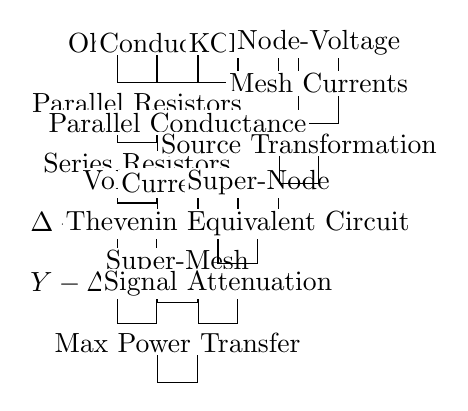
\begin{tikzpicture}[every node/.style={inner sep=0.25cm},
      tlabel/.style={fill=white,inner sep=1pt},
    ]
  
  % Ohm's Law
  \node[anchor=north west,draw=black] at (0,0) (ohm) {
    \usebox\ohmbox
  };
  \node[tlabel] at (ohm.north) {Ohm's Law};

  % Ohm's Law (Conductance)
  \node[anchor=north west,draw=black] at (ohm.north east) (conductance) {
    \usebox\conductancebox
  };
  \node[tlabel] at (conductance.north) {Conductance};

  % Kirchoff's Current Law
  \node[anchor=north west,draw=black] at (conductance.north east) (kcl) {
    \usebox\kclbox
  };
  \node[tlabel] at (kcl.north) {KCL};

  % Kirchoff's Voltage Law
  \node[anchor=north west,draw=black] at (kcl.north east) (kvl) {
    \usebox\kvlbox
  };
  \node[tlabel] at (kvl.north) {KVL};

  % Node-Voltage Method
  \node[anchor=north west,xshift=0.25cm,draw=black] at (kvl.north east) (nodevoltage) {
    \usebox\nodevoltagebox
  };
  \node[tlabel] at (nodevoltage.north) {Node-Voltage};

  % Mesh Currents Method
  \node[anchor=north west,draw=black] at (nodevoltage.south west) (meshcurrents) {
    \usebox\meshcurrentsbox
  };
  \node[tlabel] at (meshcurrents.north) {Mesh Currents};

  
  % Parallel Resistors
  \node[anchor=north west,draw=black,yshift=-0.25cm] at (ohm.south west) (parres) {
    \usebox\parresbox
  };
  \node[tlabel] at (parres.north) {Parallel Resistors};

  % Parallel Conductance
  \node[anchor=north west,draw=black,yshift=-0.25cm] at (parres.north east) (parcon) {
    \usebox\parconbox
  };
  \node[tlabel] at (parcon.north) {Parallel Conductance};

  % Series Resistors
  \node[anchor=north west,draw=black,yshift=-0.25cm] at (parres.south west) (serres) {
    \usebox\serresbox
  };
  \node[tlabel] at (serres.north) {Series Resistors};

  % Voltage Divider
  \node[anchor=north west,draw=black,yshift=-0.25cm] at (serres.north east) (vdiv) {
    \usebox\vdivbox
  };
  \node[tlabel] at (vdiv.north) {Voltage Divider};

  % Current Divider
  \node[anchor=north west,draw=black] at (vdiv.north east) (cdiv) {
    \usebox\cdivbox
  };
  \node[tlabel] at (cdiv.north) {Current Divider};

  % Supernode
  \node[anchor=north west,draw=black] at (cdiv.north east) (supernode) {
    \usebox\supernodebox
  };
  \node[tlabel] at (supernode.north) {Super-Node};

  % Source Transformation
  \node[anchor=north west,draw=black,yshift=0.75cm] at (supernode.east) (sourcetrans) {
    \usebox\sourcetransbox
  };
  \node[tlabel] at (sourcetrans.north) {Source Transformation};


  % Delta-Y
  \node[anchor=north west,draw=black,yshift=-0.25cm] at (serres.south west) (deltay) {
    \usebox\deltaybox
  };
  \node[tlabel] at (deltay.north) {$\Delta-Y$ Transform};

  % Supermesh
  \node[anchor=north west,draw=black,yshift=-0.5cm] at (supernode.south west -| deltay.north east) (supermesh) {
    \usebox\supermeshbox
  };
  \node[tlabel] at (supermesh.north) {Super-Mesh};

  % Thevenin Equivalent
  \node[anchor=north west,draw=black,yshift=-0.5cm,
    xshift=0.25cm,inner sep=0.25cm] at
  (sourcetrans.south -| supermesh.east) (thevenin) {
    \usebox\theveninbox
  };
  \node[tlabel] at (thevenin.north) {Thevenin Equivalent Circuit};
  
  % Y-Delta
  \node[anchor=north west,draw=black,yshift=-0.25cm] at (deltay.south west) (ydelta) {
    \usebox\ydeltabox
  };
  \node[tlabel] at (ydelta.north) {$Y-\Delta$ Transform};

  % Max Power Transfer
  \node[anchor=north west,draw=black,yshift=-0.5cm] at
  (supermesh.south -| ydelta.east) (maxpower) {
    \usebox\maxpowerbox
  };
  \node[tlabel] at (maxpower.north) {Max Power Transfer};
  
  % Signal Attenuation
  \node[anchor=north west,draw=black,yshift=-0.25cm] at
  (thevenin.south -| maxpower.east) (attenuation) {
    \usebox\attenuationbox
  };
  \node[tlabel] at (attenuation.north) {Signal Attenuation};
  \end{tikzpicture}

\end{my}
\begin{my}

  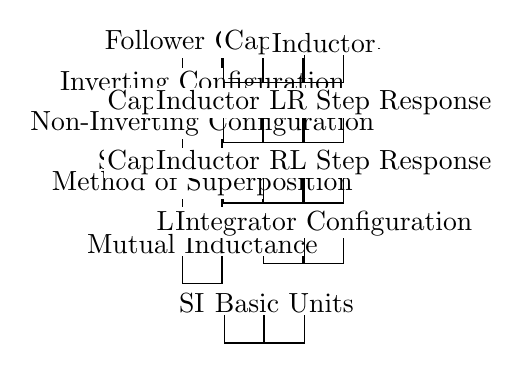
\begin{tikzpicture}[every node/.style={inner sep=0.25cm},
      tlabel/.style={fill=white,inner sep=1pt},
    ]    

  
  % Op Amp
  \node[anchor=north west,draw=black] at
  %(nodevoltage.north -| meshcurrents.east)
  (0,0) (opamp) {
    \usebox\opampbox
  };
  \node[tlabel] at (opamp.north) {Ideal Op Amp};
  
  % Inverting Configuration
  \node[anchor=north west,draw=black] at
  (opamp.south west) (inverting) {
    \usebox\invertingbox
  };
  \node[tlabel] at (inverting.north) {Inverting Configuration};
  
  % Non-Inverting Configuration
  \node[anchor=north west,draw=black] at
  (inverting.south west) (noninverting) {
    \usebox\noninvertingbox
  };
  \node[tlabel] at (noninverting.north) {Non-Inverting Configuration};
   
  % Follower Configuration
  \node[anchor=north west,draw=black] at
  (opamp.north east) (follower) {
    \usebox\followerbox
  };
  \node[tlabel] at (follower.north) {Follower Configuration};
   
  % Difference Amplifier
  \node[anchor=north west,draw=black,yshift=-0.25cm] at
  (follower.south -| inverting.east) (difference) {
    \usebox\differencebox
  };
  \node[tlabel] at (difference.north) {Difference Amplifier};
   
  % Summing Configuration
  \node[anchor=north west,draw=black,yshift=-0.25cm] at
  (difference.south west) (summing) {
    \usebox\summingbox
  };
  \node[tlabel] at (summing.north) {Summing Configuration};
   
  % Superposition
  \node[anchor=north west,draw=black,yshift=-0.25cm] at
  (noninverting.south west) (superposition) {
    \usebox\superpositionbox
  };
  \node[tlabel] at (superposition.north) {Method of Superposition};
   
   
  % Capacitor
  \node[anchor=north west,draw=black] at
  (follower.north -| difference.east) (cap) {
    \usebox\capbox
  };
  \node[tlabel] at (cap.north) {Capacitor};
   
  % Inductor
  \node[anchor=north west,draw=black] at
  (cap.north east) (ind) {
    \usebox\indbox
  };
  \node[tlabel] at (ind.north) {Inductor};
   
  % Capacitor RC Step Response
  \node[anchor=north west,draw=black,yshift=-0.25cm] at
  (cap.south west) (capstep) {
    \usebox\capstepbox
  };
  \node[tlabel] at (capstep.north) {Capacitor RC Step Response};
   
  % Capacitor CR Step Response
  \node[anchor=north west,draw=black,yshift=-0.25cm] at
  (capstep.south west) (capcrstep) {
    \usebox\capcrstepbox
  };
  \node[tlabel] at (capcrstep.north) {Capacitor CR Step Response};
  
  % Inductor RL Step Response
  \node[anchor=north west,draw=black] at
  (capcrstep.north east) (indstep) {
    \usebox\indstepbox
  };
  \node[tlabel] at (indstep.north) {Inductor RL Step Response};
   
  % Inductor LR Step Response
  \node[anchor=north west,draw=black] at
  (capstep.north east) (indlrstep) {
    \usebox\indlrstepbox
  };
  \node[tlabel] at (indlrstep.north) {Inductor LR Step Response};

  % LC Oscillator
  \node[anchor=north west,draw=black,yshift=-0.25cm] at
  (capcrstep.south west) (lc) {
    \usebox\lcbox
  };
  \node[tlabel] at (lc.north) {LC Oscillator (Ideal)};

  % LC Oscillator
  \node[anchor=north west,draw=black,yshift=-0.25cm] at
  (superposition.south west) (mutual) {
    \usebox\mutualbox
  };
  \node[tlabel] at (mutual.north) {Mutual Inductance};
  
  % Integrator Configuration
  \node[anchor=north west,draw=black] at
  (lc.north east) (integ) {
    \usebox\integbox
  };
  \node[tlabel] at (integ.north) {Integrator Configuration};
  
  
  % SI Prefixes
  \node[anchor=north east,draw=black,yshift=-0.5cm,xshift=-0.5cm] at
  (lc.south east) (prefixes) {
    \usebox\prefixbox
  };
  \node[tlabel] at (prefixes.north) {SI Prefixes};

  % Units
  \node[anchor=north west,draw=black] at
  (prefixes.north east) (units) {
    \usebox\unitsbox
  };
  \node[tlabel] at (units.north) {Basic Units};
  
 
\end{tikzpicture}
%\end{figure}
\end{my}
